\let\negmedspace\undefined
\let\negthickspace\undefined
\documentclass[journal]{IEEEtran}
\usepackage[a5paper, margin=10mm, onecolumn]{geometry}
\usepackage{tfrupee} 

\setlength{\headheight}{1cm} 
\setlength{\headsep}{0mm}     

\usepackage{gvv-book}
\usepackage{gvv}
\usepackage{cite}
\usepackage{amsmath,amssymb,amsfonts,amsthm}
\usepackage{algorithmic}
\usepackage{graphicx}
\usepackage{textcomp}
\usepackage{xcolor}
\usepackage{txfonts}
\usepackage{listings}
\usepackage{enumitem}
\usepackage{mathtools}
\usepackage{gensymb}
\usepackage{comment}
\usepackage[breaklinks=true]{hyperref}
\usepackage{tkz-euclide} 
\usepackage{listings}                                        
\def\inputGnumericTable{}                                 
\usepackage[latin1]{inputenc}                                
\usepackage{color}                                            
\usepackage{array}                                            
\usepackage{longtable}                                       
\usepackage{calc}                                             
\usepackage{multirow}                                         
\usepackage{hhline}                                           
\usepackage{ifthen}                                           
\usepackage{lscape}

\begin{document}

\bibliographystyle{IEEEtran}
\vspace{3cm}

\title{2.6.14}
\author{AI25BTECH11008 - Chiruvella Harshith Sharan}
{\let\newpage\relax\maketitle}

\renewcommand{\thefigure}{\theenumi}
\renewcommand{\thetable}{\theenumi}
\setlength{\intextsep}{10pt} 

\renewcommand{\theequation}{\arabic{equation}}
\setcounter{equation}{0}

\textbf{Question}: Find the area of the parallelogram whose diagonals are 
$\vec{d_1} = 2\hat{i} - \hat{j} + \hat{k}$ and      
$\vec{d_2} = \hat{i} + 3\hat{j} - \hat{k}$. \\\\[0.3cm]

\textbf{Solution}: \\\\[0.3cm]

The diagonals are 
\begin{align}
\vec{d_1} &= \myvec{2 \\ -1 \\ 1}, 
\quad 
\vec{d_2} = \myvec{1 \\ 3 \\ -1}.
\end{align}

\vspace{0.3cm}

The area of the parallelogram is half the magnitude of the cross product of its diagonals,
\begin{align}
A &= \frac{1}{2}\,\|\vec{d_1} \times \vec{d_2}\|.
\end{align}

Now, using the identity
\begin{align}
\|\vec{d_1} \times \vec{d_2}\|^2 
= \|\vec{d_1}\|^2 \|\vec{d_2}\|^2 - (\vec{d_1}\cdot \vec{d_2})^2,
\end{align}
we compute
\begin{align}
\|\vec{d_1}\|^2 &= 2^2 + (-1)^2 + 1^2 = 6, \\
\|\vec{d_2}\|^2 &= 1^2 + 3^2 + (-1)^2 = 11, \\
\vec{d_1}\cdot \vec{d_2} &= (2)(1) + (-1)(3) + (1)(-1) = -2.
\end{align}

Hence,
\begin{align}
\|\vec{d_1} \times \vec{d_2}\|^2 &= (6)(11) - (-2)^2 \\
&= 66 - 4 = 62.
\end{align}

\[
\implies \|\vec{d_1} \times \vec{d_2}\| = \sqrt{62}.
\]

Finally,
\[
A = \frac{1}{2}\sqrt{62}.
\]

\begin{figure}[htbp]
    \centering
    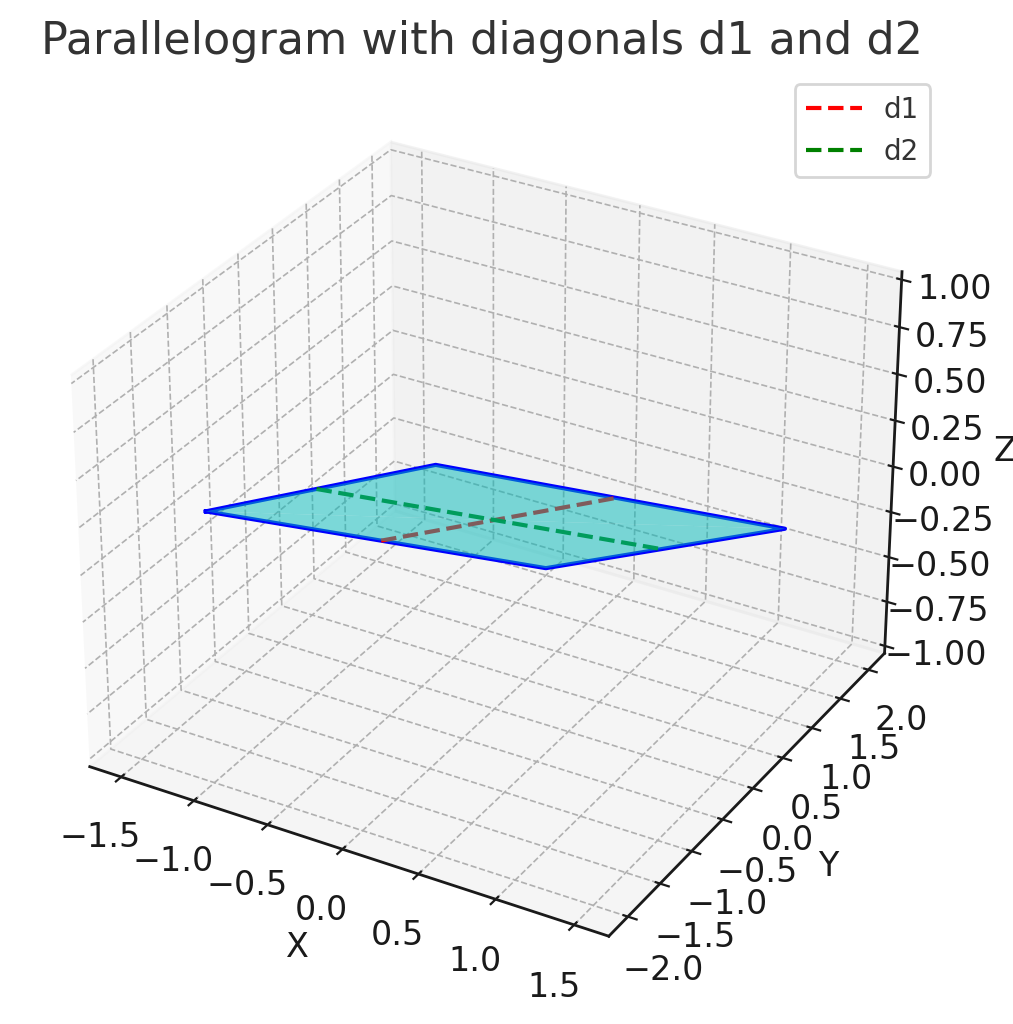
\includegraphics[width=0.8\linewidth]{figs/fig1.jpg}
    \caption{}
    \label{fig:fig/fig1.png}
\end{figure}

\end{document}
